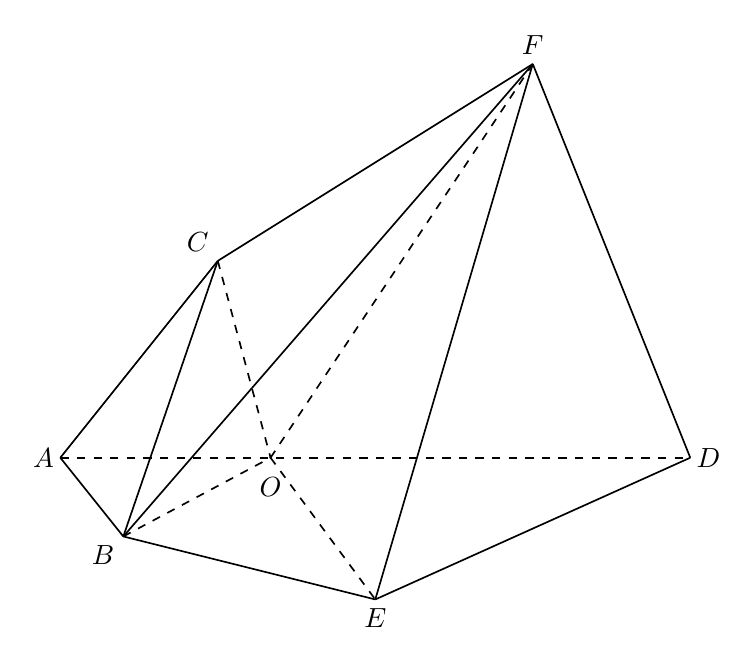
\begin{tikzpicture}[x=1cm,y=1cm,font=\normalsize,line width=.6pt]
\coordinate (A) at (0,2);
\coordinate (O) at (2.67,2);
\coordinate (D) at (8,2);
\coordinate (B) at (0.8,1);
\coordinate (C) at (2,4.5);
\coordinate (E) at (4,0.2);
\coordinate (F) at (6,7);
% base axis AD (hidden)
\draw[dashed] (A) -- (D);
% left triangles
\draw[solid] (A) -- (B);
\draw[solid] (A) -- (C);
\draw[solid] (B) -- (C);
% lower part
\draw[solid] (B) -- (E);
\draw[solid] (E) -- (D);
% right part
\draw[solid] (F) -- (D);
\draw[solid] (F) -- (E);
\draw[solid] (F) -- (C);
\draw[solid] (F) -- (B);
% hidden segments through O
\draw[dashed] (B) -- (O);
\draw[dashed] (C) -- (O);
\draw[dashed] (O) -- (E);
\draw[dashed] (O) -- (F);
\node[left,inner sep=2pt] at (A) {$A$};
\node[below left,inner sep=3pt] at (B) {$B$};
\node[above left,inner sep=3pt] at (C) {$C$};
\node[below,inner sep=3pt] at (E) {$E$};
\node[right,inner sep=2pt] at (D) {$D$};
\node[above,inner sep=3pt] at (F) {$F$};
\node[below,inner sep=2pt,yshift=-5pt] at (O) {$O$};
\end{tikzpicture}
